\documentclass[aspectratio=169]{beamer}
\usepackage{amsmath, amssymb, amsfonts, amsthm}
\usepackage{lmodern}
\usepackage{cancel}
\usepackage[output-complex-root=j]{siunitx}
\usepackage[american, nooldvoltagedirection]{circuitikz}
\usepackage{bm}
\usepackage{listings}
\usepackage{graphicx}
\usepackage{hyperref}

\usetheme{Berkeley}
\usefonttheme[onlymath]{serif}
\AtBeginSection[]{
    \begin{frame}
    \vfill
    \centering
    \begin{beamercolorbox}[sep=8pt,center,shadow=false,rounded=false]{title}
    \usebeamerfont{title}\insertsectionhead\par
    \end{beamercolorbox}
    \vfill
    \end{frame}
}

\newcommand{\N}{\mathbb{N}}
\newcommand{\Z}{\mathbb{Z}}
\newcommand{\Q}{\mathbb{Q}}
\newcommand{\R}{\mathbb{R}}
\renewcommand{\C}{\mathbb{C}}
\newcommand{\tpose}[1]{\left[#1\right]^{\! \top} \!\!}

\title{EECS 16B CSM}
\author{Bryan Ngo}
\date{2020-10-25}
\institute{UC Berkeley}

\begin{document}

\begin{frame}
    \maketitle
\end{frame}

\section{Stability}

\begin{frame}
    \frametitle{Continuous}
    
    \centering
    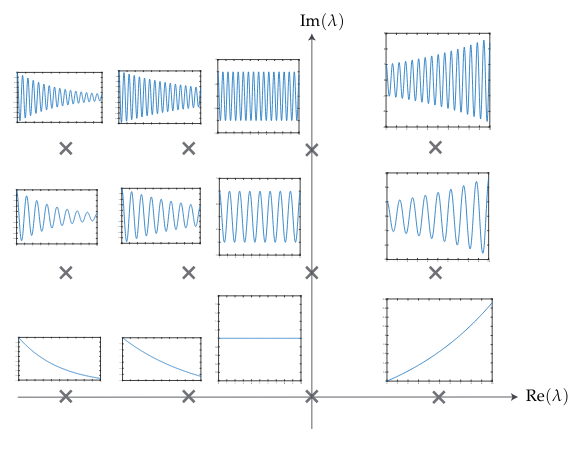
\includegraphics[width=\textheight]{../2020-10-19/continuous.png}
\end{frame}

\begin{frame}
    \frametitle{Discrete}
    
    \centering
    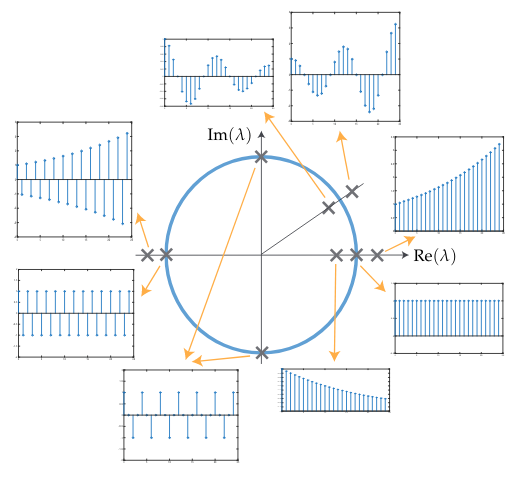
\includegraphics[width=\textheight]{../2020-10-19/discrete.png}
\end{frame}

\section{Feedback}

\begin{frame}
    \frametitle{Open-Loop}

    \begin{equation}
        \bm{x}[t + 1] = \bm{Ax}[t] + \bm{Bu}[t]
    \end{equation}

    \begin{itemize}
        \item define a certain range of use
        \item simpler
        \item no restraints apart from stability
    \end{itemize}
\end{frame}

\begin{frame}
    \frametitle{Closed-Loop}

    \begin{align}
        \bm{u}[t] &=
        \begin{bmatrix}
            k_1 & k_2 & \cdots & k_n
        \end{bmatrix}
        \begin{bmatrix}
            x_1[t] \\
            x_2[t] \\
            \vdots \\
            x_n[t]
        \end{bmatrix} \\
        \bm{x}[t + 1] &= \bm{Ax}[t] + \bm{BKx}[t] = (\bm{A} + \bm{BK}) \bm{x}[t]
    \end{align}

    \begin{itemize}
        \item adaptable to a wide range of use
        \item more complex
        \item self-correcting
        \item requires more constraints
    \end{itemize}
\end{frame}

\begin{frame}
    \frametitle{Controller Canonical Form}

    \begin{align}
        \bm{x}[t + 1] &=
        \begin{bmatrix}
            0 & 1 & 0 & \cdots & 0 \\
            0 & 0 & 1 & \cdots & 0 \\
            \vdots & \vdots & \vdots & \ddots & \vdots \\
            0 & 0 & 0 & \cdots & 1 \\
            a_1 & a_2 & a_3 & \cdots & a_n
        \end{bmatrix} \bm{x}[t] +
        \begin{bmatrix}
            0 \\
            0 \\
            0 \\
            \vdots \\
            1
        \end{bmatrix} \bm{u}[t] \\
        \det(\bm{A} + \bm{BK} - \lambda \bm{I}) &= \lambda^n - \sum_{i = 1}^n (a_i + k_i) \lambda^i
    \end{align}
\end{frame}

\section{Least Squares}

\begin{frame}
    \frametitle{Quick Review}

    \begin{equation}
        \bm{Ax} = \bm{b} \implies \bm{\hat{x}} \approx (\tpose{\bm{A}} \bm{A})^{-1} \tpose{\bm{A}} \bm{b}
    \end{equation}
    \begin{itemize}
        \item we want to minimize the error vector \(\bm{e} = \bm{b} - \bm{Ax}\)
    \end{itemize}
\end{frame}

\end{document}
